\problem{Homomorphic Filtering}
The Homomorphic filter is:
$$H(u,v)=(\gamma_H-\gamma_L)*\left[1-\exp\left(-c\left[\dfrac{D(u,v)}{D_0}\right]^2\right)\right]+\gamma_L$$
Where
$$\gamma_L<1,\gamma_H\geq 1,D(u,v)=\left[\left(u-\dfrac{P}{2}\right)^2+\left(v-\dfrac{Q}{2}\right)^2\right]^\frac{1}{2}$$

In this specific situation, we take $\gamma_L = 0.5, \gamma_H = 2.0, D_0 = 80, c = 1$.

In order to do FFT, we need to pad the image to the size of $2^m*2^n$, where $m$ and $n$ are integers.

So the images size varies: $1162*746\Rightarrow 2048*1024$.

And aftering filtering, the image is cropped to the original size.

The Homomorphic filter is shown in \ref{fig:p2_filter}.
\begin{figure}[htbp]
    \centering
	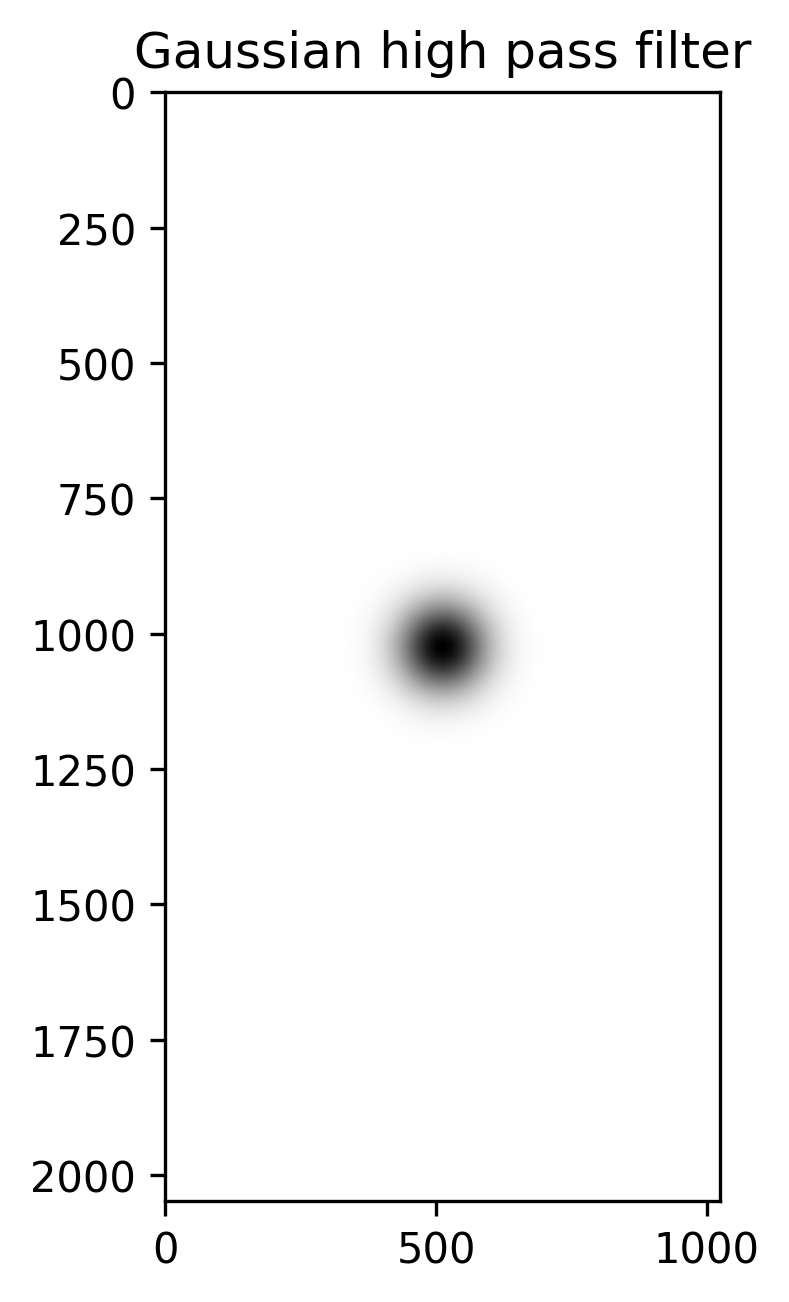
\includegraphics[width=0.49\textwidth]{../images/p2/p2a_filter.png}
	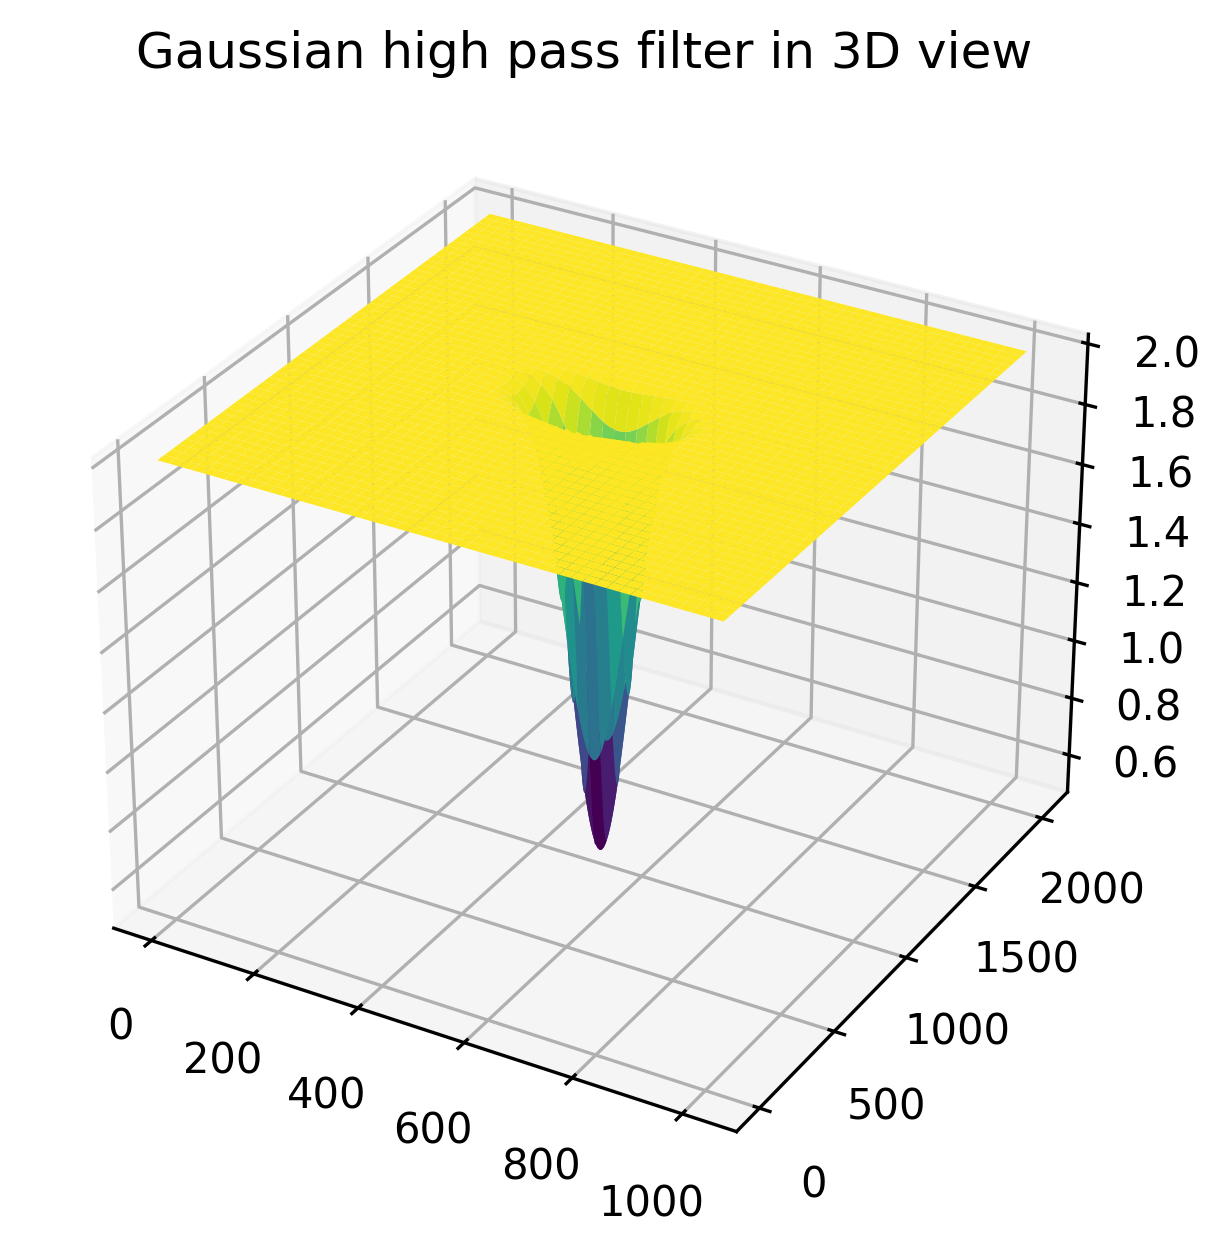
\includegraphics[width=0.49\textwidth]{../images/p2/p2a_filter_3D.png}
    \caption{Homomorphic filter}
    \label{fig:p2_filter}
\end{figure}
\\

The results of filtering the image with the Homomorphic filter is shown in Figure \ref{fig:p2_result}.

The variance of pixel values with in the white box $[500, 1100]\times[90, 180]$ is $0.0017427355$, which exceeds $3\times 10^{-4}$.\\



\begin{figure}[htbp]
    \centering
	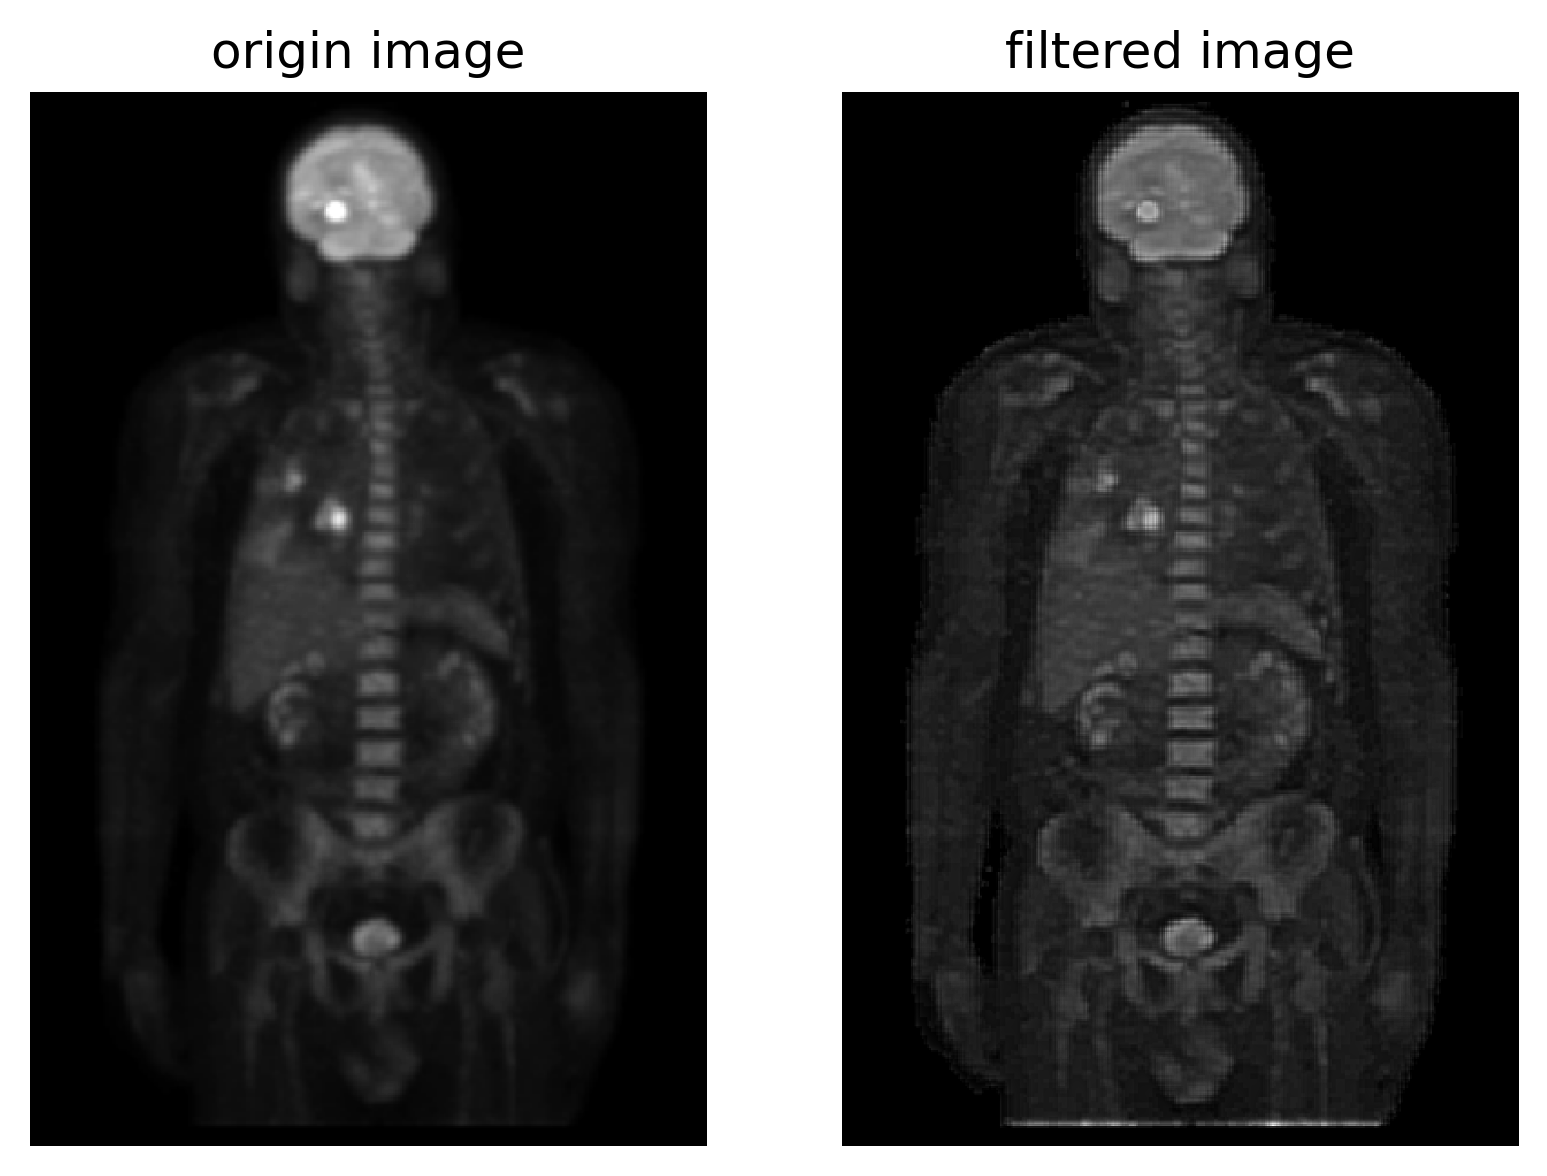
\includegraphics[width=\textwidth]{../images/p2/p2a_result.png}
    \caption{Result after Homomorphic filtering}
    \label{fig:p2_result}
\end{figure}




\newpage